\documentclass{article}
\usepackage[utf8]{inputenc}
\usepackage{natbib}
\usepackage{graphicx}
\usepackage{float}
\usepackage{url}
\usepackage{commath}

\title{Realtime Environment Lighting Simulation for Augmented Reality  Applications}
\author{Marco Antonio Salcedo Sanson }
\date{February 2017}

% Definition of \maketitle
\makeatletter         
\def\@maketitle{
\noindent
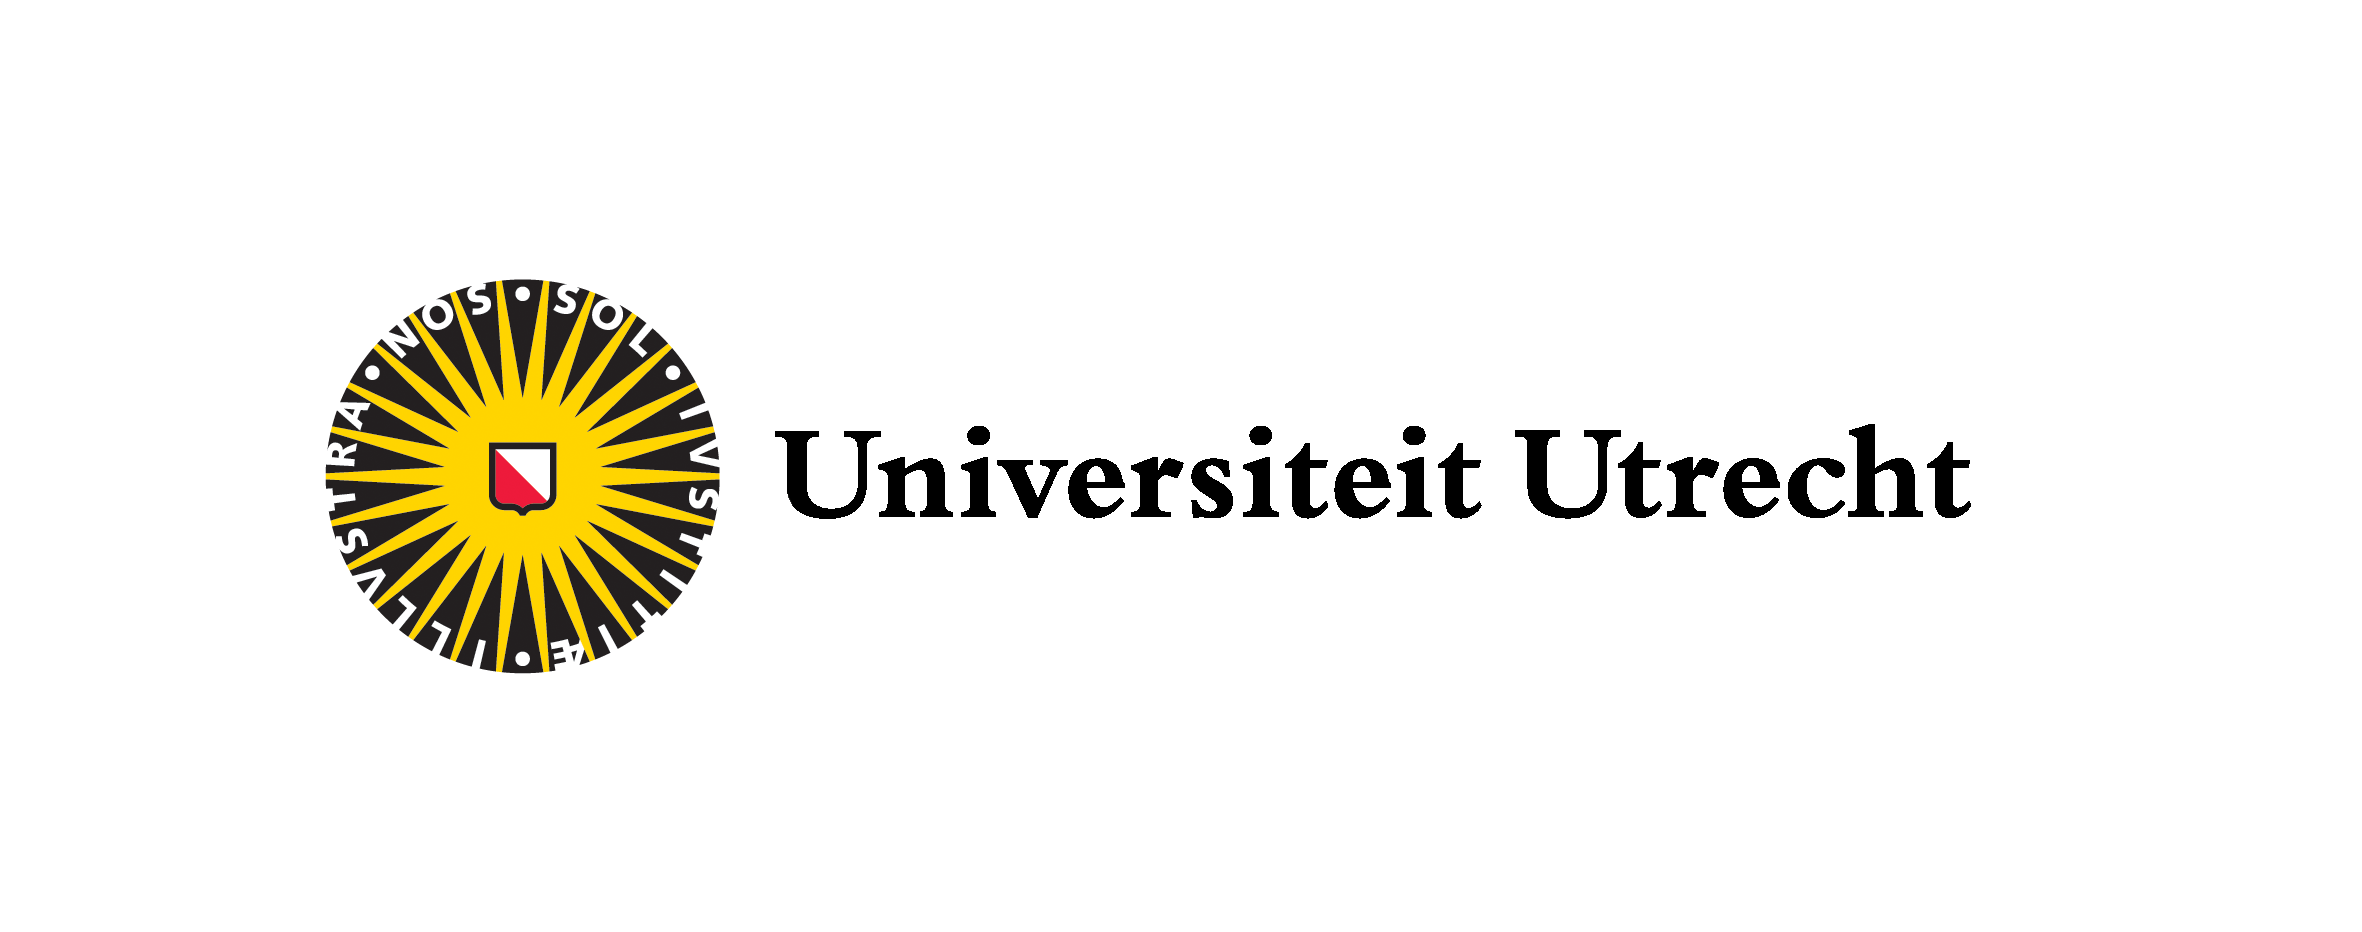
\includegraphics[scale = 0.5]{Figures/uu-logo.png}\\[8ex]
\begin{center}
{\huge \bfseries \sffamily \@title }\\[4ex] 
{\Large  \@author}\\[4ex] 
\@date\\[8ex]
\end{center}}
\makeatother


\begin{document}

\maketitle

\section{Introduction}
The rendering of virtual objects on current AR applications has a number of shortcomings in the state of the art. It is quite easy to tell that it’s a superimposed virtual object. There are many factors that come into play and give away the lack of feasibility of an AR object, such as marker jiggle, inaccurate depth cues, lack of occlusion from real life objects and incompatible lighting.
The method proposed in this work addresses the latter problem, the non-matching light conditions of the virtual and real world. The method is based on the idea that a 360 photograph of the environment can give us a lot of information about the lighting conditions and that such 360 photographs are now simple to create on an average mobile device. From this 360 photograph it can be determined if the environment is outdoors by day or any other case of illumination. If the environment is indoors the light sources of the room will be approximated using the photo, if outdoors the sun will be assumed as the main source of light, and its position would be calculated using the clock, calendar and compass of the mobile device running the application. \newline
Whatever the case, the method's output is a set of lights whose properties are a position relative to the camera, a rotation and an intensity.
It's important to stress the fact that the method is proposed for mobile devices. There have been previous works, as detailed in the next section, that deal with the same problem but on computers. Mobile devices present advantages over computers for this task, but also the downside of generally lower processing power compared to computers. This decision comes from the ease of producing the 360 photographs locally, from the judgement that AR is better suited for mobile devices than computers (for mobility and ease of use reasons) and also to be able to exploit the devices geolocation hardware. Of course this doesn't mean that the method will only be applicable to mobile, there are also ways to adapt it to work on computers too.\newline
The research question from which this method was originally envisioned is: "Can the accuracy of lighting in AR applications be improved using a mobile device to it's full potential?". What this means is that thanks to the many ways a smartphone or tablet can interact with the user and the environment we can know a lot about the surroundings. And this information could potentially be very useful to save computation time, which is the main downside to using mobile devices, their relatively lower computational capabilities.\newline
The contributions of this method are:
\begin{itemize}
    \item An image-based method with which the lighting conditions of the full visible environment can be modeled
    \item The use of the mobile device's geolocation hardware to enhance the light simulation with the knowledge of the current weather conditions and the position of the sun
\end{itemize}


\section{Related Work}
Agusanto et al. proposed a similar method \cite{agusanto2003}. The main differences in the method they propose have to do mostly with the technologies used. Being already an old paper, their method was conceived for Augmented Reality on a computer, rather than on a smartphone. My choice of a smartphone comes with the downside of lower processing power, but with the great advantage of the different sensors available on the device. The method in the Agusanto paper infers the lighting conditions using hand-crafted HDR photographs of the real scene using highly reflective metal spheres in contrast with my proposition of using the 360 degree photograph on the device itself, which is a lot more accessible to an average consumer.\newline
Pessoa\cite{pessoa2011} expanded on Agusanto's work and created the Real-Time Photorealistic Rendering of Synthetic Objects into Real Scenes (RPR-SORS) toolkit as an extension of the ARToolkit Augmented reality SDK. Although they use more modern techniques, such as cubemaps instead of HDR photographs, their approach still has the same differences than the Agusanto method.\newline
There have been several methods to insert virtual objects into static photographs automatically with highly realistic results. One such example is the method by Karsh \cite{karsh2014} These kind of methods are not suitable for real- time applications, and they use a single view image to infer the lighting conditions. The method proposed here is more robust in the sense that it uses a 360 view of the environment to eliminate assumptions of what there is out of frame.\newline
Xing\cite{xing2013} also devised a method to compose virtual objects into static photographs, focusing on outdoors scenes. The method is quite sophisticated, but a lot of the information fed to the light calculation functions involve manual input by the user. The proposed method is intended to work both for indoors and outdoors scenes, the main difference with the way outdoors scenes will be managed is that the method works automatically, without user intervention. This is accomplished by the usage of the mobile device's dedicated geolocation hardware. By using it, there is no need to assume anything or ask for any user input, the device will be able to tell a good approximation of the sun position using only the sensor's information.

\section{Theoretical Framework}
In this section a few technical concepts will be explored in order to make the proposed method and what it aims to accomplish more clear.

\textbf{Augmented Reality}\newline
As of yet, the definition of Augmented Reality that is most widely accepted is the one presented by Azuma\cite{azuma1997}. In this survey Augmented Reality (or AR for short) is defined as a software system that features a blend of real and virtual objects, the user can interact with it in real time and presents a 2D representation of a 3D world for both the real and virtual sides. A feature film that integrates real and virtual characters or objects is therefore strictly speaking not AR for example, because it's static content, the consumer cannot interact with it at all, let alone in real time.
In order to combine real and virtual objects both worlds must be aligned, in the sense that they must share a common origin for both position and rotation. If the virtual objects present in the real scene are not aligned the feasibility of the whole composition is compromised. The tracking of real world features as a guideline for alignment in the virtual world is one of the challenges in the field of AR. There are many techniques that have been used, such as sensor-based tracking, that uses dedicated hardware to feed the software application the position and rotation information it needs; vision-based tracking, in which the position and orientation origin of the virtual world are determined by images recognized by a computer vision algorithm. These images are named fiducial markers and can be an artificial black and white image, a "natural" images (points, lines, shapes and/or textures) or even 3D objects. Other approaches involving both sensors and vision algorithms have also been used, if the reader is interested in learning more about tracking, Zhou's survey\cite{zhou2008} on tracking is a good resource.
This method does not aim in any way to improve tracking for AR, current state-of-the-art methods will be used for that, but it's important to explain the concept a bit in order to settle the scope and expectations of the end result.

\textbf{Sensors}\newline
Most smartphones and tablets in the market nowadays have built-in sensors to measure many things that are helpful for application developers, such as motion, orientation and other environmental conditions. The ones that are relevant for this method are the following:\newline
\textbf{Accelerometer}: This device measures proper acceleration relative to gravity. Its application in mobile development is to measure motion changes and to measure the device orientation relative to Earth's surface. It usually consists of 3 orthogonal axes. The output is given in m/s\textsuperscript{2} \newline
\textbf{Gyroscope}: A sensor that is capable of measuring the rate of rotation around a particular axis. It serves the same purpose as the accelerometer, but mobile devices usually have both for more robust measurements. The output is given in rad/s. In the method these will be used to acquire the 360 panoramic photograph, making sure that the device is within the same pitch while capturing all the images that will be stitched together to make the panorama. \newline
\textbf{Photometer}: There is a wide variability in terms of capacity of photometers across different devices, but the only measurement that is guaranteed is the ambient illuminance expressed in lx.  In the method it will be useful for detection of a noticeable change in ambient lighting, leading to a re-capture of the panorama. What exactly constitutes a noticeable change in ambient lighting will be determined through parameter tuning. \newline 
\textbf{Magnetometer}: In terms of mobile devices it serves the purpose of a compass, it measures the device's orientation with respect to the Earth's magnetic poles. In mobile development it is useful to get the heading of the device expressed in degrees.\newline
\textbf{GPS}: Measures the raw position of the device in three-dimensional Cartesian coordinates with origin on the center of the Earth. It can be used to determined where on planet Earth the device is located (Country, city, neighborhood, etc). It needs to have line of sight with no electromagnetic interference with at least 4 out of the 24 satellites in orbit that are used for GPS. \newline

\section{Method}
This section covers the steps needed to produce the wanted results. The input needed is a fiducial marker M to provide the object position in the real world; and a 3D mesh O which will be rendered in Augmented Reality. The output is a set of light sources L\textsubscript{i}, each one having a position, orientation, intensity, color and size. In order to complete the luminance (luma) analysis a 360 panoramic image is required, but it will be generated as a previous step, it is not necessary to have one beforehand. The entirety of the process is layed out in the flowchart in Figure 1, and each step is described in more detail afterwards.

\begin{figure}[H]
  \centering
  \setlength{\unitlength}{\textwidth} 
    \begin{picture}(1,0.5)
       \put(-0.1,0){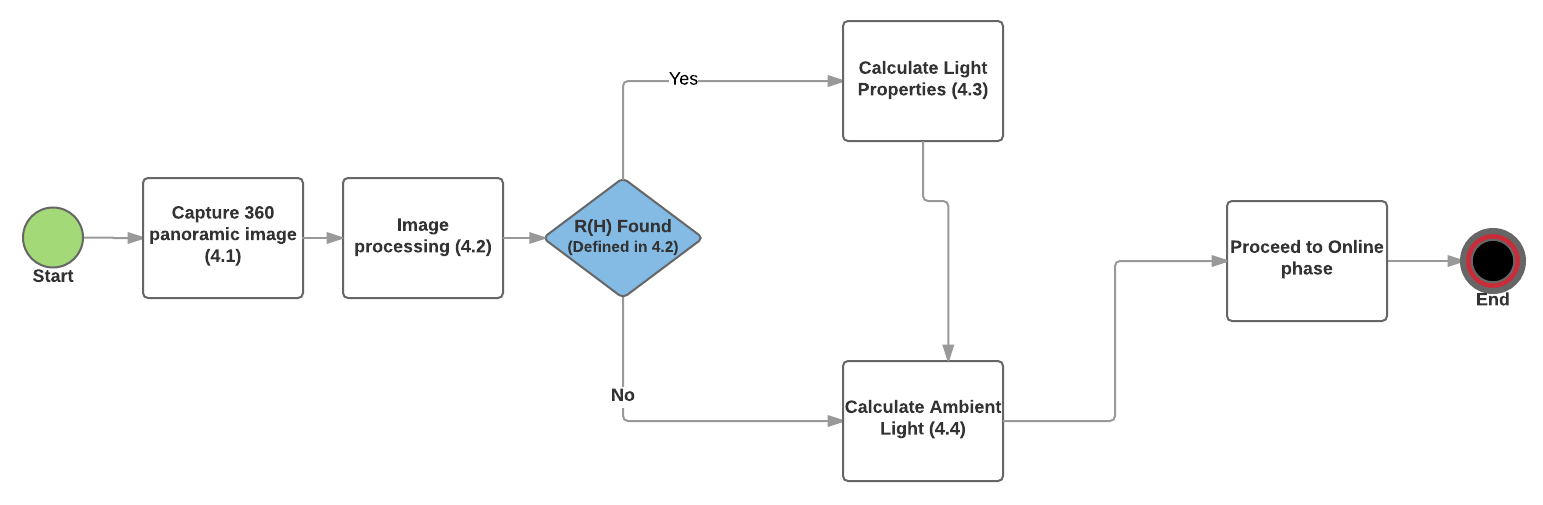
\includegraphics[width=1.3\unitlength]{Figures/Flowchart.png}}
       
    \end{picture}
    \caption{The method in a nutshell}
\end{figure}

\subsection{Panoramic image capture}
In this work panoramic images are used as a tool, therefore it's not within the scope of the method to define a new way of capturing 360 images. The implementation will be based on the one by Chuang et al. \cite{ThreeSixty}
In order to simplify the calculation of light parameters later on, a modification to their implementation will be done forcing the user to face north when beginning to take the panoramic capture.

\subsection{Image processing}
Once the panoramic image exist the first step in order to be able to analyze the luminance is to get rid of the chrominance information. This is achieved by desaturating the image. The contrast ratio has to be adjusted, so that the regions with high luminance are more clearly differentiable. The result of these steps is a black and white image with the rough shape of the light source. If the image ends up completely black it means there are no important visible light sources and ambient illumination alone would give a good enough result on the rendered model. A region of high luminance is defined as follows:
\[
    R(H) = \{p_{00}, p_{01}, ... , p_{mn}\}
\]
 Where p\textsubscript{ij} is the pixel in the i,j position of the image. Such that 
\[
    L(p_{ij}) > 0.9 \times max(L(p_{ij})) 
\]
However if there are regions of high luminance they would be discovered with a fair amount of noise and artifacts, caused by clear objects, reflections of light sources on highly reflective surfaces, or even light sources that are so far away in the distance that don't really contribute an important amount of light to the area of interest. Therefore it's necessary to also add a relative size constraint to the definition. What constitutes an acceptable region size to deem the light source is not an easy question to answer. The best approach to face this problem is to define it as a percentage of the width and height of the overall image and tune the parameter in search for the best solution. The size constraint would therefore be:

\[
    width(R(H)) \times height(R(H)) \geq k \times W \times H
\]
Where k is the parameter to be tuned; W and H are the total image width and height.\newline

These constraints also help keep the amount of lights to be processed within an acceptable range for a real-time application, even if the real environment has many light sources a simplification of them is necessary when modelling them to keep the application feasible. Once the relevant light sources have been identified their properties need to be calculated.

\subsection{Calculate light properties}
The properties needed to calculate for each light are position, orientation, intensity, size and color. In the real world there is no way to calculate the position and size at the same time, because at least one of them would have to be known. Fortunately in the virtual world this is not necessary, as long as it is consistent, for the area size of the light the pixel measures can be used. With this in mind all the other properties can be calculated.

\begin{enumerate}
\item Width and height: The pixel measures will be used for this, they can me determined from the size constraint in the previous step.
\item Position: It is posible to calculate the distance from and object to a camera lens knowing a few parameters from the lens, namely the focal lenght and the sensor size. In Android these values are easily obtainable through the ExifInterface class. In iOS the values are publicly known per device family, so it's possible to create a lookup table with the values and have the application ask what device it's running on to match the necessary set of values. The calculation is then done as follows:
\[
    d(L_i) = \frac{ f \times h_i}{sensorHeight}
\]
\item  Orientation: Since the user was enforced to capture the environment starting from the north and the environment is the entire 360 degrees it is easy to map the pixel width to the angle of incidence of the light source. We can for example define the following ratio to calculate the angle:
\[
    \phi = \frac{pos(L_i)_x \times 180}{imageWidth \times 0.5}
\]
\item Color: Storing both versions of the panorama, one in full color and another one after processing will allow us to have both the color and the luminance information. Once a light source is detected, the equivalente area in the color image can be averaged to determine the color of the light source.
\end{enumerate}

\subsection{Calculate ambient light}
Since the data from the device's sensors are available something more involved than having a default value of ambient illumination for the entire scene. Ambient illumination when no visible light sources are present is more often than not due to sunlight, be it in an outdoors scene or coming in from a window somewhere. There are ways \cite{solar} to calculate the sun position in spherical coordinates using the latitude, longitude, time of the day and day of the year of the observer. This information can be easily retrieved using the devices GPS, clock and calendar. The direction in which the sunlight is affecting the scene can be used in a per-vertex illumination shader to adjust the amount of ambient light in a specific vertex of the virtual object. This contribution can be done using lambertian diffuse contribution:
\[
    I_a = K_a \times (N \cdot L)
\]
Where $K_a$ is the maximum ambient contribution, N is the vertex normal and L is the light direction vector, normalized.
\section{Expected results}
In this section the measure of success and the scope of the method will be described. In terms of scope the aim of the method is to produce plausible lighting for Augmented Reality applications, and thus increase the sense of realism of the composed graphics. This does not mean that imagery that would for all practical purposes be indistinguishable from reality will be achieved. As said earlier, the non-matching lighting is only one of the problems with current AR graphics. In order to achieve complete realism all the other problems would have to be tackled as well, this includes occlusion from real objects as the most prominent one, but also the shadows of real objects not affecting the virtual ones at all. The method will also not attempt to improve other aspects of AR, such as tracking. The method comprises an offline and an online phase, offline being the acquisition of the 360 panorama and it's analysis for calculation; online is the actual rendering. It is also desirable and expected that the offline phase can be completed within a reasonable time frame on a mobile device, in terms of usability this should be no more than 1 minute.\newline
Since the final product is a graphic on a screen, an image, it's somewhat difficult to define a measure of success, due to the inherent subjective nature of image appreciation. It can be said that the method successfully converged if in the final image the synthetic objects are hard to tell from the real ones, if formed on a line on a still image. Hard to tell meaning that some scrutiny and reflection is necessary when looking at a screen capture of the application. If an average technology consumer is able to immediately tell which of the objects are synthetic and which are real the method will then have failed. To explain the measure better in Figure 2 we can see three objects, 2 real, 1 synthetic, from an AR included with the Vuforia library. Figure 3 shows the same array of objects, again the same 2 real and 1 synthetic, but in this case the synthetic object having been inserted with hand tuned lighting. It can be appreciated that it is harder to differentiate the virtual object in the second image than on the first one.
\begin{figure}
\centering
\includegraphics[width=0.6\textwidth]{Figures/fake.jpg}
\caption{Default lighting, making the virtual object stand out}
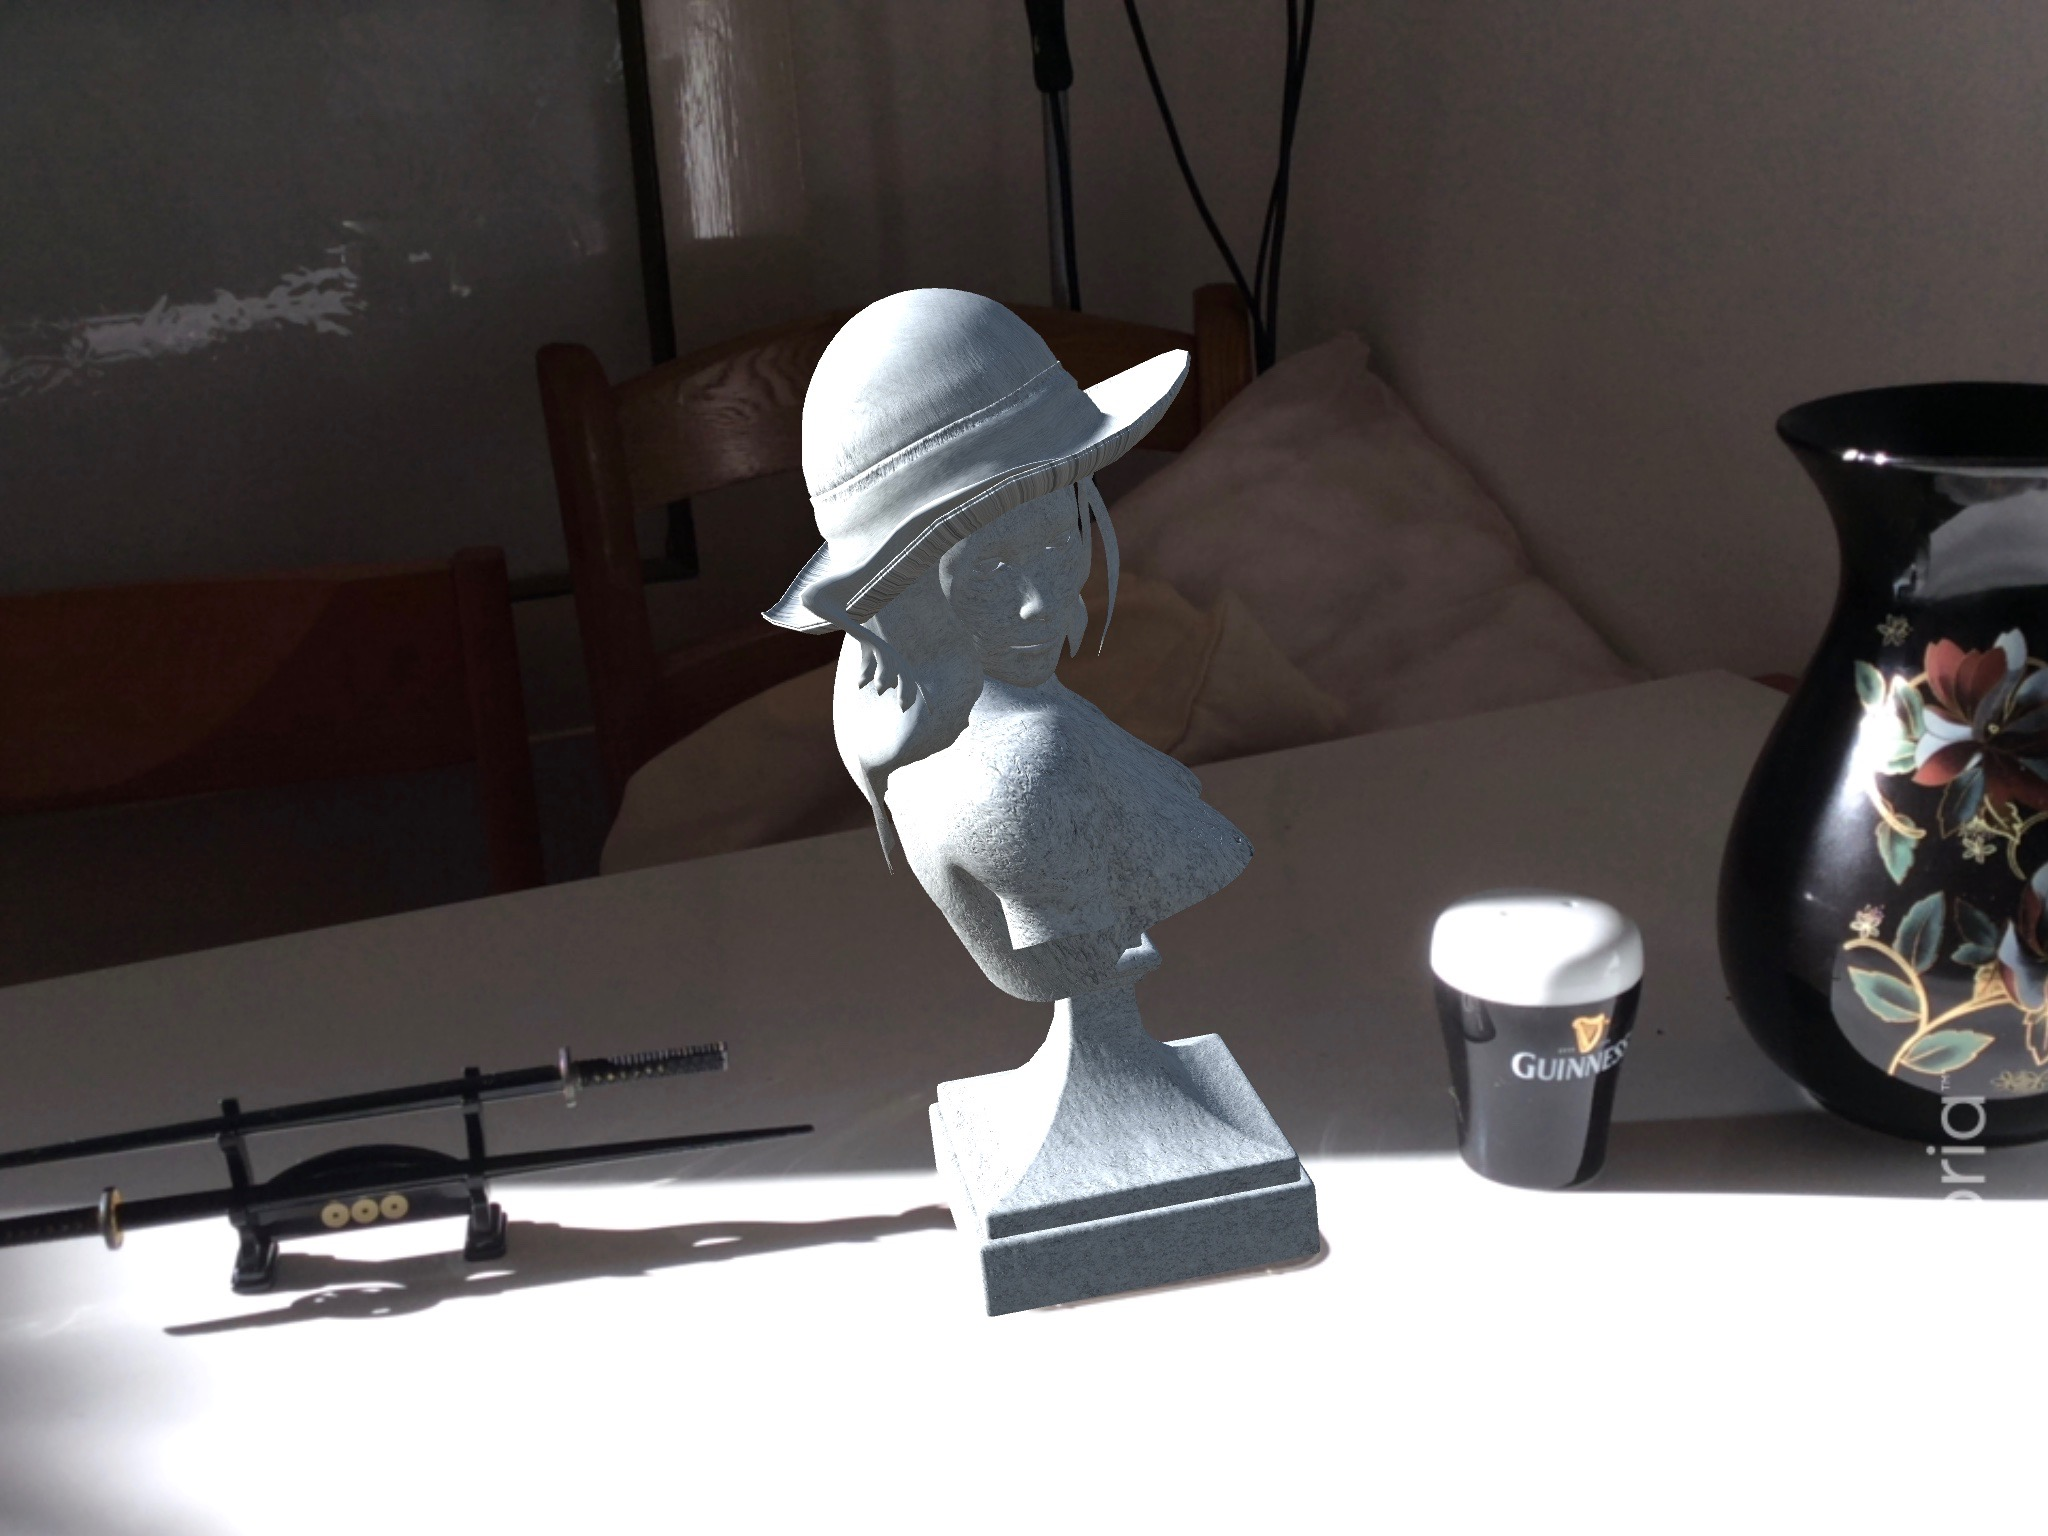
\includegraphics[width=0.6\textwidth]{Figures/realish.jpg}
\caption{Adjusted lighting, giving a more believable look}
\end{figure}


\clearpage

\section{Conclusion}
The above discussion has highlighted the potential benefits of using a mobile device's hardware in a smart way to obtain information about the environment and be able to produce a more convincing lighting estimation than what's currently available in AR applications. Unlike previous works reviewed, this method is conceived for mobile devices and real-time applications, while also being as user-friendly as possible, in the sense of keeping user interaction to a bear minimum and obtaining information that's already available through the hardware. 

\bibliographystyle{plain}
\nocite{*}
\bibliography{references}
\end{document}
